\chapter{Diseño de \rc}

% Software Design
\textit{Diseñar} es el proceso de planificar y resolver problemas de un software en particular. Una vez que el propósito y las
especificaciones del software están determinados, debemos desarrollar un plan para llegar a una solución. Para llevarlo a cabo se incluyen
tanto la especificación de los diferentes módulos (o componentes) bien detallados, lo que llamamos \textbf{diseño de bajo nivel}, así como
el punto de vista arquitectónico o estructural, conocido como \textbf{diseño de alto nivel}.

\section{Diseño de Alto Nivel}

Desde el punto de vista de la ingeniería de software, el diseño de software es una etapa crucial del desarrollo de software, en la cual sus
implicaciones y deficiencias afectan el proyecto a lo largo de su ciclo de vida \cite{pressman}, por lo que la toma de decisiones sobre el
diseño es una tarea que debe ser llevada a cabo con especial atención y cuidado.

En esta tesis se emplearon \textit{principios de diseño de software}, los cuales representan un conjunto de directrices que nos ayudan a
evitar tener un mal diseño. Los principios de diseño se asocian a \textit{Robert Martin}, quien los reunió en el libro \textit{``Agile
Software Development: Principles, Patterns, and Practices''} \cite{martin-asd}. Según el autor, hay tres características importantes de un
mal diseño que deben evitarse:
\begin{itemize}
    \item   \textbf{Rigidez}: es difícil modificar porque cada cambio afecta a muchas otras partes del sistema.
    \item   \textbf{Fragilidad}: cuando hacemos un cambio, partes inesperadas del sistema se rompen.
    \item   \textbf{Inmovilidad}: es difícil reutilizar componentes en otra aplicación, ya que no se pueden desligar de la aplicación
            actual.
\end{itemize}
        
Para evitar estas \textit{malas} características, se intentó que el diseño cumpliese los principios fundamentales del diseño de software,
comúnmente conocidos por el acrónimo ``\textbf{SOLID}''\cite{objmentor} (\textbf{S}ingle responsibility, \textbf{O}pen-closed,
\textbf{L}iskov substitution, \textbf{I}nterface segregation y \textbf{D}ependency inversion). Aplicando estos principios de manera
conjunta, hacen más probable que un programador construya un sistema fácil de mantener y extensible en el tiempo.
\begin{description}
    \item   \textbf{Single Responsibility Principle (SRP)}: No debe existir más de una razón para que una clase cambie. Esto significa
            que una clase con diferentes responsabilidades debe ser dividida en clases más simples.
    \item   \textbf{Open-Closed Principle (OCP)}: Este principio establece que las entidades de software (clases, módulos, funciones,
            etc.) deben estar abiertas para su extensión pero cerradas para su modificación\cite{oosc}.
    \item   \textbf{Liskov Substitution Principle (LSP)}: Aquellas funciones que usan punteros o referencias a clases base deben ser capaces
            de utilizar objetos de clases derivadas, sin saberlo. Barbara Liskov lo describió unos 8 años antes \textit{Barbara Liskov} en
            el articulo \textit{``Data Abstraction and Hierarchy''} \cite{Liskov:1987:KAD:62139.62141} como:
            \begin{quote}
                \textit{Lo que se intenta aquí es algo como la siguiente propiedad de sustitución: Si para cada objeto o$_1$ de tipo S
                existe un objeto o$_2$ de tipo T tal que para todos los programas P definidos en t\'ermino de T, el comportamiento de P no
                se ve alterado cuando o$_1$ es sustituido por o$_2$, entonces S es un subtipo de T.}
            \end{quote}
    \item   \textbf{Interface Segregation Principle (ISP)}: Los clientes no deben ser forzados a depender de interfaces que no usan, lo que
            puede ser interpretado como el hecho de que las interfaces deben tener usuarios que las usen de manera completa, no parcial. Si
            este último fuese el caso, entonces debe haber otra interfaz con el subconjunto de métodos que este usuario particular
            necesita.
    \item   \textbf{Dependency Inversion Principle (DIP)}: Este principio establece dos puntos:
            \begin{itemize}
                \item   Módulos de alto nivel no deben depender de módulos de nivel más bajo. Ambos deben depender de abstracciones.
                \item   Abstracciones no deben depender de los detalles. Los detalles deben depender de las abstracciones.
            \end{itemize}   
\end{description}

Observando el diagrama OSI del framework \fud(\ref{sisd}) se puede observar claramente que el diseño se divide en dos partes, aplicaciones
cliente y servidor. A su vez, cada una de estas partes se encuentra organizada en 3 capas separadas, donde cada una de ellas posee una
responsabilidad bien definida.

%%%%%%%% ADD theories about client-server architecture. %%%%%%%%

Cabe destacar que el único enlace \textit{real} entre las aplicaciones cliente y servidor estará en el nivel más bajo, es decir, en
alguna implementación del \textit{middleware} de distribución (L1). Las restantes formas de comunicación son abstractas y deben
atravesar la estructura de capas.

\subsection{Arquitectura de \rc{} sobre \fud}

En la figura \ref{recabs_layers} se encuentra el diagrama al estilo OSI de redes donde se muestra una aplicación concreta, de solución
recursiva que es resulta usando \rc, el cual está montado sobre \fud. Este montaje respeta su arquitectura original (Véase
\ref{fud_layers}), agregando una nueva capa superior. En el mismo se muestran los componentes más importantes de este proyecto así como
también los mas relevantes del framework.

\begin{figure}[ht]
    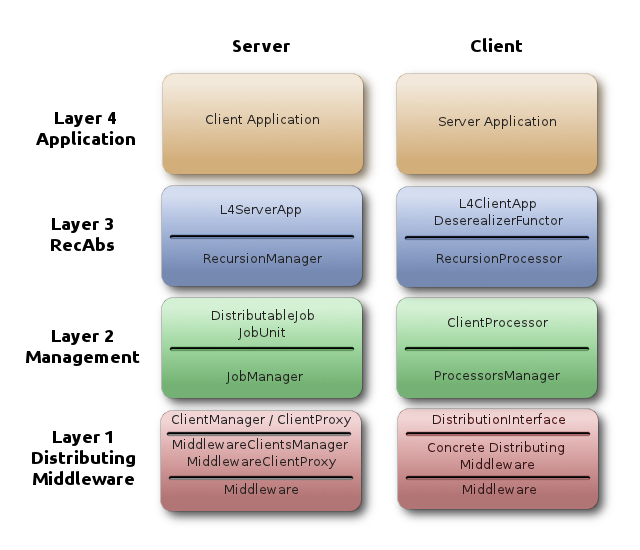
\includegraphics[scale=.6]{images/recabs.png}
    \caption{Capas de \texttt{RecAbs} + \texttt{FuD}}
    \label{recabs_layers}
\end{figure}

\subsection{Aplication Layer (L4)}

La ``capa aplicación'' proporciona los componentes que contienen todos los aspectos del dominio del problema en cuestión. Entre estos
aspectos se incluyen todas las definiciones de datos que se usan y la manipulación de los mismos, como así también, los algoritmos
relevantes para la solución del problema.

Es necesario aclarar que esta capa no forma parte de \rc(L3) ni del framework \fud(L2 y L1), así como cualquier código de aplicación que
usa una librería no forma parte de la misma. La inclusión de esta capa al diseño tiene como propósito la comprensión de cómo una aplicación
utiliza la biblioteca y, por lo tanto, el funcionamiento de la misma.

Para mantener la arquitectura cliente-servidor, esta capa se separa en lado cliente, lado servidor y también una parte común a ambos lados:
\begin{itemize}
    \item   \textbf{Lado Servidor}.\\
            Es necesario proveer a la capa subyacente el \textit{functor recursivo} inicial de la aplicación, y ademas, definir que hacer  
            con los mensajes intermedios y resultados que van llegando al servidor. Ver \ref{server_helper}.
    \item   \textbf{Lado Cliente}.\\
            Se necesitan proveer estos requerimientos:
            \begin{itemize}
                \item   la deserialización de un \textit{functor recursivo} a partir de los paquetes enviados de servidor a clientes. Para
                        ello, se cuenta se cuenta con MiLi, particularmente los \textit{binary streams}, que son de gran utilidad en
                        \textit{serialización} y \textit{deserialización} de paquetes.
                \item   la cantidad y el tiempo en que se envían mensajes o resultados desde el cliente hacia el servidor. Para ello se
                        cuenta con un interfaz e implementaciones concretas o bien, permite la propia que el usuario desee implementar (ver
                        \ref{client_helper}).
                \item   opcionalmente, se puede especificar una política de distribución propia, la cual establece cuándo y cuántas unidades
                        de trabajo se deben distribuir, dependiendo del estado en que se encuentre el servidor. Para más detalles vea
                        \ref{distribution_policy}.
            \end{itemize}
    \item   \textbf{Parte común}.\\
            Se debe proveer, a la capa L3, la definición de un \textit{functor recursivo} específico al problema que L4 desee atacar, por lo
            que básicamente se deben declarar cuáles son sus atributos necesarios y la serialización del mismo. Como se menciono en         
            \ref{functor}, un \textit{functor} representa a la función que el creador de la aplicación L4 desea distribuir a sus clientes
            para el posterior procesamiento en cada uno de ellos.
\end{itemize}


\subsection{\rc{} Layer (L3)}

Esta es la capa que provee el ``molde'' para definir soluciones a problemas que requieren un modelo recursivo (sin dependencias
horizontales dentro del árbol de recursión, ver \ref{problem_desc}) y, al mismo tiempo, provee una solución algorítmicamente
eficiente para dichos proyectos.

Siguiendo el mismo esquema de separación según la arquitectura cliente-servidor, las principales responsabilidades de esta capa son:
\begin{itemize}
    \item   \textbf{Lado Servidor}.\\
            La responsabilidad de esta capa es iniciar y administrar la recursión que haya propuesto la aplicación L4, y más
            específicamente, el servidor es el encargado de mantener una \textit{pila} de functores (nodos del árbol de recursión) que
            representa a los nodos que no han sido procesados todavía. De esta manera la capa subyacente solo deberá \textit{apilar} cuando
            llegue un nuevo nodo para procesar o \textit{desapilar} cuando se quiera obtener el próximo nodo para enviar a un cliente
            ocioso.

            Otra responsabilidad que toma el server es la de notificar a la capa superior de la llegada de mensajes y resultados, dejando
            el tratamiento de éstos como métodos a implementar.

            El servidor es el que inicia la recursión con el \textit{functor} inicial que es creado por la aplicación (L4).
    \item   \textbf{Lado Cliente}.\\
            El cliente es el encargado de realizar la ejecución total (o parcial) del functor que le fue asignado. Para cumplir su función
            se suple de las siguientes funcionalidades:
            \begin{itemize}
                \item   Deserialización de functores.
                \item   Descomposición del problema en más functores, de los cuales, si es posible, serán redistribuidos para repartir el
                        trabajo en varios clientes. Este paso comúnmente se apoya en un middleware de distribución HPC (en nuestro caso
                        \fud).
                \item   Política de distribución de functores, el cuál nos dirá cuándo y cuánto trabajo debemos
                        distribuir para que otros
                        clientes trabajen, y de esta forma balancear la carga de trabajo para cada cliente.
                \item   Envío de resultados o mensajes según la política que se use: enviar cada un determinado tiempo, cada tantos
                        bytes de memoria, etc.
            \end{itemize}

            Todo esta maquinaria hace que \textit{un} cliente procese sus resultados sin sobrecargar demasiado al servidor, permitiendo     
            distribuir functores que no estén siendo atendidos por él a clientes ociosos.
    \item   \textbf{Parte común}.\\
            Tanto el servidor como los clientes tienen la noción de estado de un \textbf{\textit{functor}}, el cual representa el estado
            particular de una función recursiva, y su función primordial es la de auto-reproducirse: genera una lista de sus functores
            hijos. Cuando se desee utilizar algún middleware de distribución, se manipula un tipo especial de \textit{functor}, el cuál
            además de las funciones mencionadas anteriormente, se le agrega la capacidad de serializarse, lo que permite una representación
            homogénea que todo cliente pueda deserializar llegado el momento de hacerlo.
\end{itemize}

\subsection{Diagrama de clases de \rc}

Para tener una visión macroscópica sobre el diseño de alto nivel, en la figura \ref{class_diagram} se presenta el \textit{diagrama de
clases} de \rc, el cuál netamente es sólo la capa de abstracción para soluciones recursivas (L3), acompañado de sus capas inmediatas: por un
lado está la capa subyacente (L2) que simboliza la parte alta del framework de distribución \fud, y por otro lado la capa superior (L4) la
cuál representa una aplicación que usa la librería \rc.

\begin{center}
    \begin{landscape}
        \begin{figure}[ht]
            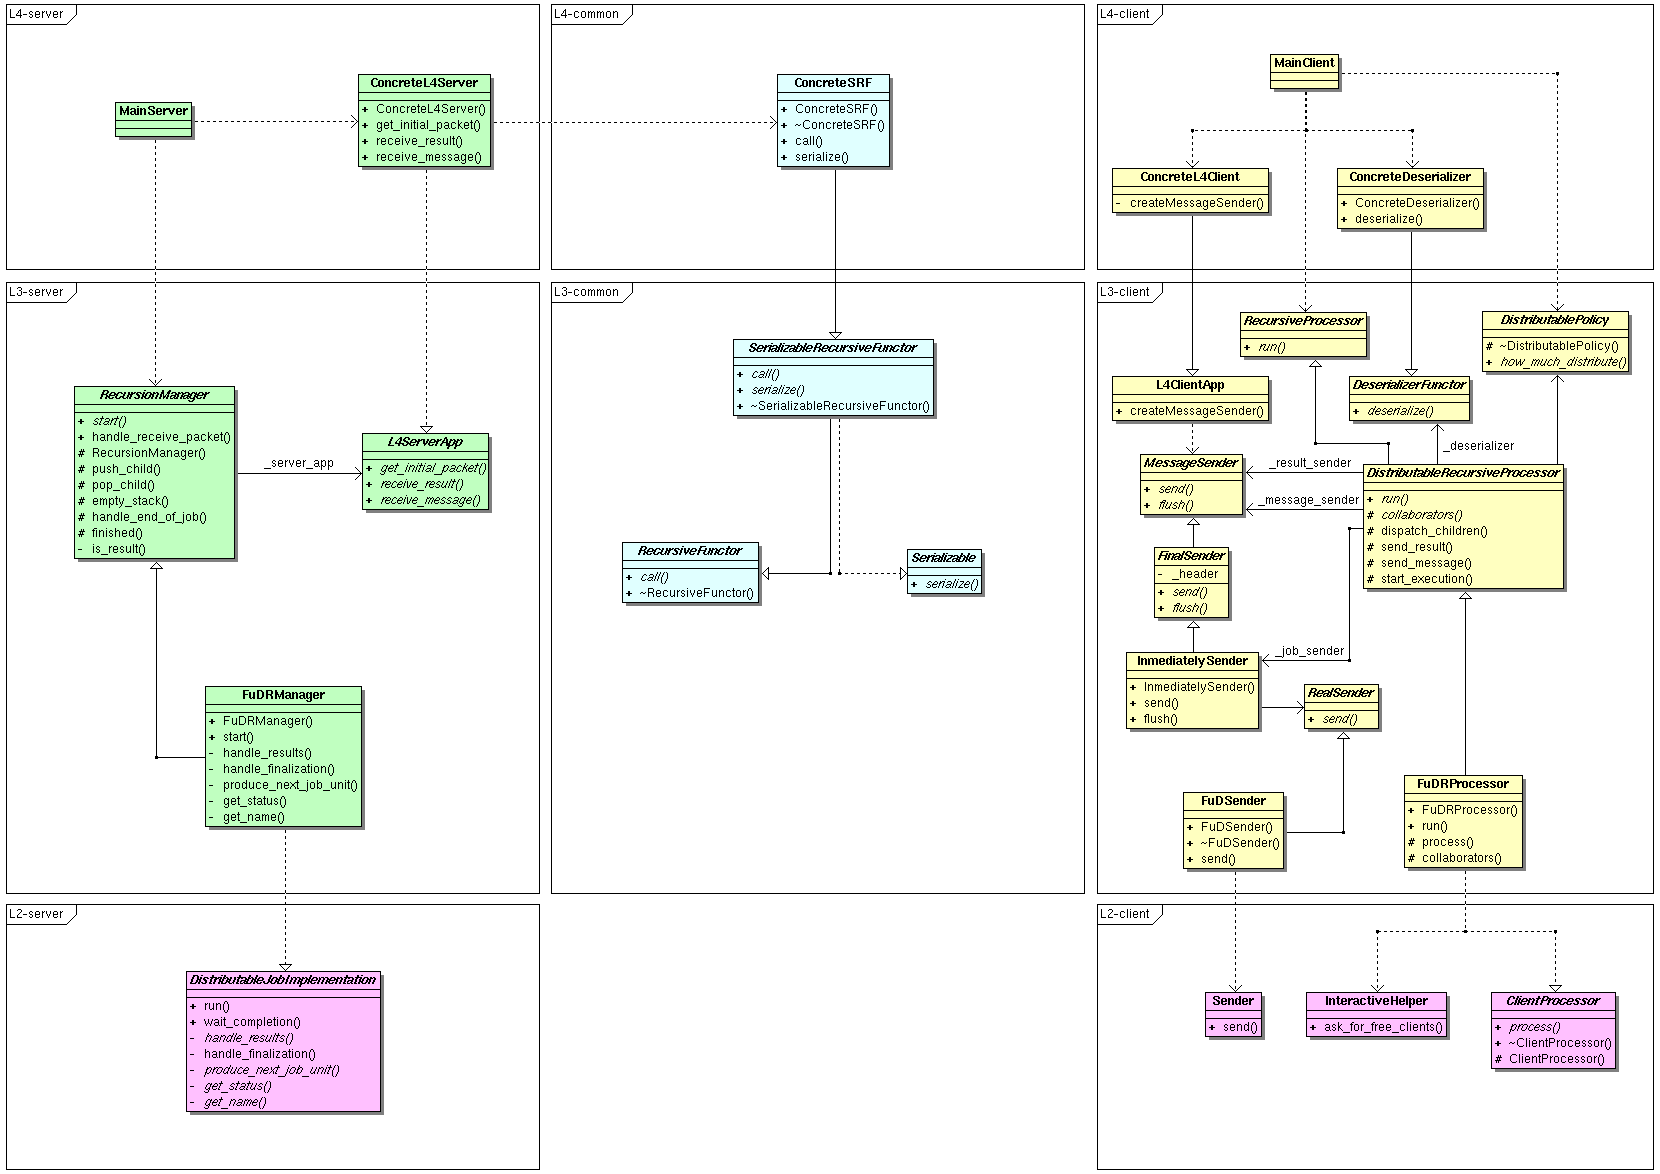
\includegraphics[scale=.35]{images/class.png}
            \caption{Diagrama de clases de \rc \ y sus capas inmediatas}
            \label{class_diagram}
        \end{figure}
    \end{landscape}
\end{center}


\section{Diseño de Bajo Nivel}

Aquí se hace un refinamiento de las decisiones de diseño sobre aquellos componentes abstractos presentes en el
diseño de alto nivel. Además, se analiza cómo estas clases están compuestas: los atributos de cada una, los métodos que
declaran y sus interacciones con el resto del sistema. 

A continuación se describen los módulos mas importantes de la capa \rc{}, detallando las decisiones tenidas en
cuenta a la hora de diseñarlos. Para cada componente del módulo se muestra un diagrama de clases
simplificado.

\subsection{Functor Recursivo}

Anteriormente se describió abstractamente el concepto de un Functor Recursivo. Con el fin
de modelar este concepto se estableció esta jerarquía de clases:
    
    \subsubsection{\texttt{RecursiveFunctor}}
        Todo functor es representado por una implementación de la interfaz \\ \texttt{RecursiveFunctor} que publica el
        método \texttt{call}. Por tanto, una aplicacion concreta deberá implementar este método dando creación a un
        nuevo \textit{functor} que representará la función que el usuario desee distribuir.

        \begin{figure}[ht] \hspace{4.5cm}
            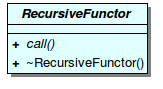
\includegraphics[scale=.75]{images/rf.png}
            \caption{Clase \texttt{RecursiveFunctor}}
        \end{figure}
        
    \begin{itemize}
        \item \texttt{call(ChildrenFunctors\& children, Packet\& result, WhenToSend\& when)}
               Este método deberá encapsular el comportamiento de la función recursiva a modelar de manera que se
               especifiquen el contenido de los parámetros de la siguiente forma:
        \begin{description}
            \item[children] Rellenar con los functores resultantes de un paso de la recursión del proceso.
            \item[result]   Aquí va un mensaje hacia el servidor, puede ser de dos tipos según el momento del
                            procesamiento en el que se encuentre. En caso de estar en el final de un nodo, o sea en
                            el caso base, donde \texttt{children} será una lista vacía, el mensaje deberá contener el
                            resultado ya serializado. De esta manera \texttt{message} será enviado al servidor y
                            tratado como como un resultado final del nodo corriente. Pero en el caso de que el nodo este
                            en medio de una rama y se quiera enviar un mensaje a la aplicación lado servidor se
                            puede usar este parámetro para notificar mediante un mensaje serializado, por ejemplo,
                            el estado actual el procesamiento.
            \item[when] Mediante un tipo enumerado, especificar el momento del envío del mensaje o resultado. Esto
                        puede ser \texttt{kSendThisImmediately}, el cual indica que el mensaje sea enviado
                        inmediatamente; \\ \texttt{kSendAllImmediately} indica que el mensaje sea enviado inmediatamente
                        junto con el resto de los mensajes en espera y por ultimo \texttt{kSendWhenRecAbsWants} donde se
                        le otorga a \rc{} la responsabilidad de enviarlo cuando éste lo disponga.
        \end{description}
    \end{itemize}

    \subsubsection{\texttt{SerializableRecursiveFunctor}}

        Es la versión serializable de la clase descrita anteriormente, es decir hereda directamente de
        \texttt{RecursiveFunctor} agregando un método extra también puro virtual para proporcionar la
        funcionalidad de serialización y permitir el envío de estos functores a través de algún middleware de
        distribución.

        \begin{figure}[!htb] \hspace{3.8cm}
            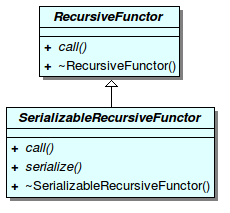
\includegraphics[scale=0.75]{images/srf.png}
            \caption{Clase \texttt{SerializableRecursiveFunctor}}
        \end{figure}
   
    \begin{itemize}
        \item \texttt{void serialize(Packet\& pkt)}

        Aquí un functor concreto deberá implementar la serialización, especificando de que manera el objeto es
        empaquetado en \texttt{pkt}
    \end{itemize}


\subsection{Asistente del Servidor}

Ya habíamos introducido en \ref{server_helper} las responsabilidades de este asistente. Se realizó una interfaz que
será implementada por el desarrollador de una aplicación, especificando métodos necesarios para iniciar la ejecución del
servidor y para asimilar los resultados arrojados.

\subsubsection{\texttt{L4ServerApp}}

Esta interfaz brindará el \textit{functor} inicial y definirá que se hará con los resultados y mensajes intermedios a medida que
lleguen. Ver clase en figura \ref{l4_server_app}.

\begin{figure}[ht] \hspace{4.8cm}
    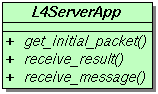
\includegraphics[scale=.68]{images/l4_server_app.png}
    \caption{Clase \texttt{L4ServerApp}.}
    \label{l4_server_app}
\end{figure}

\begin{itemize}
    \item \texttt{void get\_initial\_packet(Packet\& pkt)}\\[0.2cm]
                Deberá retornar (en el parámetro \texttt{pkt}) un paquete de datos que represente al \textit{functor} inicial de la
                aplicación. Debido a que este \textit{paquete} es la serialización de un \textit{functor}, las clases hijas tendrán una
                relación con el \texttt{RecursiveFunctor} del problema corriente. Dado el ejemplo de la figura
                \ref{l4_server_app_with_srf}, ver que una implementación concreta de \texttt{L4ServerApp} necesariamente deberá ``conocer''
                al \texttt{SerializableRecursiveFunctor} concreto para poder crear el \textit{functor} inicial y luego llamar al método
                \texttt{serialize()}, el cual lo retorna como un paquete. Dicho paquete inicial será enviado a un cliente, para que sea éste
                quién inicie la ejecución  de la aplicación.
    \item \texttt{void receive\_result(const Packet\& result)}\\[0.2cm]
                Durante el procesamiento de un \textit{functor}, los clientes pueden enviar resultados al servidor. Éste método es el que
                define que se harán con los mismos.
    \item \texttt{void receive\_message(const Packet\& msg)}\\[0.2cm]
                Durante el procesamiento de un \textit{functor}, los clientes pueden enviar mensajes intermedios al servidor. Éste método es
                el que define que se harán con los mismos. Cabe aclarar, que a diferencia de los resultados, éstos pueden ser enviados en
                cualquier momento de la etapa de recursión, y no, como los resultados, sólo en las hojas pertenecientes al árbol de
                recursión, generado por el \textit{functor} ejecutado.
\end{itemize}

\begin{figure}[ht] \hspace{1.8cm}
    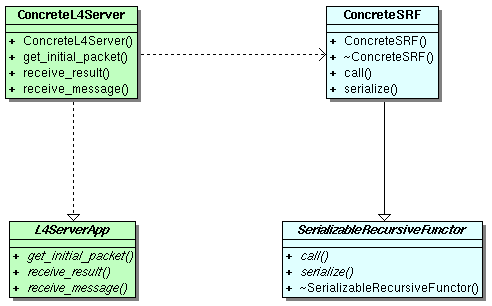
\includegraphics[scale=.6]{images/l4_server_app_with_srf.png}
    \caption{Colaboración \texttt{L4ServerApp} - \texttt{SerializableRecursiveFunctor}.}
    \label{l4_server_app_with_srf}
\end{figure}


\subsection{Administrador de recursión}
    Es quién organiza y manipula los functores pendientes del proceso recursivo, interactúa con el middleware de
distribución para tal propósito. Para más detalles de sus responsabilidades véase la sección \ref{rmanager}.

\subsubsection{\texttt{RecursionManager}}

Es la clase que modela un \textit{administrador de recursión}. En la figura \ref{recursion_manager} está graficada su entidad.

\begin{figure}[ht] \hspace{4.7cm}
    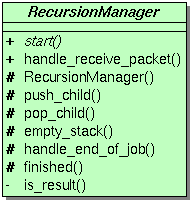
\includegraphics[scale=.6]{images/recursion_manager.png}
    \caption{Clase \texttt{RecursionManager}.}
    \label{recursion_manager}
\end{figure}

Las \textit{unidades de trabajo} se mantienen en una pila, la cual se va desapilando a medida que haya usuarios ociosos. Debido a ello, la
clase cuenta con un basto número de operaciones que manejan esta pila, y también posee métodos que conocen de la finalización de la
ejecución total de la aplicación y del cómputo de cada \textit{functor}.

\texttt{RecursionManager} tiene el método \texttt{start()} que deja como abstracto para las posibles implementaciones según el middleware
que se utilice en la capa subyacente. Este método deberá iniciar la ejecución total de cualquier proyecto que use la librería.

Para realizar su trabajo cuenta con la colaboración de la interfaz \texttt{L4ServerApp}, el cuál nos brinda el functor inicial, que es dado
al primer cliente dando así la iniciación del proceso recursivo, y es el procesador de resultados y mensajes de los clientes que computan
sus funciones.

\begin{figure}[ht] \hspace{1.5cm}
    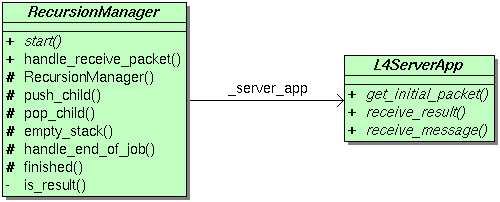
\includegraphics[scale=.6]{images/rec_manager_with_l4_server_app.png}
    \caption{Colaboración \texttt{RecursionManager} - \texttt{L4ServerApp}.}
    \label{rec_manager_with_l4_server_app}
\end{figure}


\subsubsection{\texttt{FuDRManager}}

Es el administrador de recursión específico del framework de distribución \fud. Como dijimos anteriormente, este implementa la rutina
\texttt{start()} y de esta forma es una realización concreta del administrador de recursión. Cabe aclarar que esta clase es un ``sabor'',
una posible implementación, no es la única, y cada concretización de un \textit{manager} dependerá del modelo de distribución que se quiera
utilizar en la capa inferior. Como resultado de este montaje, las aplicaciones correrán sobre el framework \fud{} implementando métodos de
\texttt{DistributableRecursiveProcessor}. Véase \ref{fud_manager_dji}.

\begin{figure}[ht] \hspace{4.5cm}
    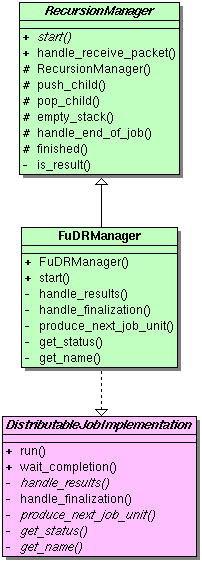
\includegraphics[scale=.6]{images/fud_manager_dji.png}
    \caption{Clase \texttt{FuDRManager}.}
    \label{fud_manager_dji}
\end{figure}


\subsection{Procesador Recursivo}

Este módulo representa el engine de ejecución recursiva, es decir, es el cerebro del procesamiento local en un
nodo de un functor recursivo. Fué diseñado con una jerarquía de \texttt{processors} donde cada uno va
adhiriendo responsabilidades con el fin de permitir otras implementaciones de este engine sin mucho costo de
acoplamiento.
    
    \subsubsection{\texttt{RecursiveProcessor}}

        Interfaz que representa el engine genérico publicando el método \texttt{run}, el cual deberá
        implementar todo procesador concreto. Ver \ref{rp}.

        \begin{figure}[ht] \hspace{4.8cm}
            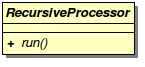
\includegraphics[scale=0.75]{images/rp.png}
            \caption{Clase \texttt{RecursiveProcessor}}
            \label{rp}
        \end{figure}
        
        \begin{itemize}
            \item \texttt{void run(const Address\& address = LOCALHOST, Port port = DEFAULT\_PORT)}
                Método responsable de iniciar el proceso en un nodo de procesamiento.
                \begin{description}
                \item[address] IP del servidor.
                \item[port] el puerto del servidor.
                \end{description}
        \end{itemize}

    \subsubsection{\texttt{DistributableRecursiveProcessor}}

        Es la versión \textit{distribuible} de
        \texttt{RecursiveProcessor}, agregando funcionalidad de interacción con el servidor de modo que pueda consultar
        sobre disponibilidad, enviar trabajos incompletos, enviar mensajes o resultados al servidor.
        Ésta clase también engloba a toda implementación de un procesador que necesite distribución de trabajos, por
        tanto si bien provee toda la maquinaria para lograr la distribución, deja libre a cualquier plataforma de
        comunicación la implementación del middleware, por tanto delega la definición del método \texttt{run}. (Véase
        \href{DistributableRecursiveProcessor})

        \begin{figure}[ht] \hspace{3.8cm}
            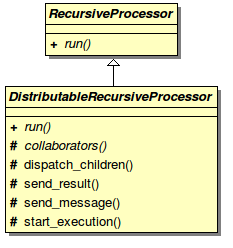
\includegraphics[scale=0.75]{images/drp.png}
            \caption{Clase \texttt{DistributableRecursiveProcessor}}
            \label{DistributableRecursiveProcessor} 
        \end{figure}

%         \begin{itemize}
%             \item \footnotesize{\texttt{virtual void start\_execution(const Packet\& init\_packet))}}\\
% 
%             \item \footnotesize{\texttt{void do\_recursion(ChildrenFunctors\& functor\_list)}}
% 
%             \item \footnotesize{\texttt{void reproduce(RecursiveFunctor* rf, ChildrenFunctors\& functor\_list)}}
% 
%             \item \footnotesize{\texttt{void send\_result(const Packet\& packet, WhenToSend when)}}
% 
%             \item \footnotesize{\texttt{void send\_message(const Packet\& packet, WhenToSend when)}}
%         \end{itemize}

        
    \subsubsection{\texttt{FuDRProcessor}}

        Es el procesador recursivo distribuible concreto que en parte monta al cliente \rc{} sobre el cliente \fud{}.
        Implementa el método \texttt{run} de \\ \texttt{DistributableRecursiveProcessor} el cual será invocado una sola
        vez al comienzo del procesamiento nodal. Es una pieza fundamental en el montaje con \fud{} ya que describe a
        \rc{} como una aplicación que correrá sobre el framework implementando métodos de \texttt{ClientProcessor}.
        (Véase \ref{FuDRProcessor})
    
        \begin{figure}[ht] \hspace{4.2cm}
            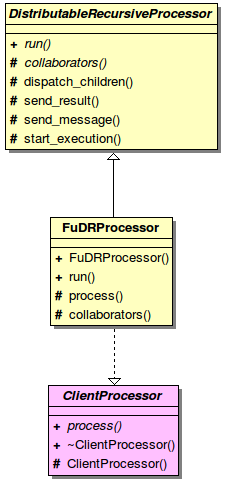
\includegraphics[scale=0.70]{images/frp.png}
            \caption{Clase \texttt{FuDRProcessor}}
             \label{FuDRProcessor}
        \end{figure}


\subsection{Deserializador}

Cuando un functor arriba a un cliente, éste se encuentra codificado para que el servidor pudiese enviarlo.
Es responsabilidad de este módulo de especificar de que manera se realiza el método inverso a la serialización
realizada en el lado servidor. Por cada functor concreto se tendrá que implementar esta deserialización.

    \subsubsection{\texttt{DeserializerFunctor}}
        Interface que publica el método puro virtual \texttt{deserialize}

        \begin{figure}[!htb] \hspace{4.8cm}
            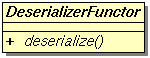
\includegraphics[scale=0.70]{images/deserializer.png}
            \caption{Clase \texttt{DeserializerFunctor}}
             \label{Deserializer}
        \end{figure}

        \begin{itemize}
            \item \texttt{deserialize(const Packet\& p, SerializableRecursiveFunctor** rf)}

                Método que será invocado por \texttt{DistributableRecursionProcessor} al incio del procesamiento local.
                \begin{description}
                \item[p]: Es el functor enviado por el server ya serializado.
                \item[rf]: Aquí se deberá dejar el functor ya deserializado.
                \end{description}
        \end{itemize}
    
    
\subsection{Senders}

    Aquí se define la lógica de tratamiento de mensajes (tanto mensajes propiamente dichos como resultados) antes de
ser enviados al servidor. Lo cual implica definir con que middleware de distribución se harán los envíos así como
también los diferentes criterios de manipulación. Para lograr esto se usó el patrón \textit{Chain of Responsibility}
(\textit{Véase} \ref{chain_pattern}) ya que se brinda al usuario final la posibilidad de encadenar distintos senders
ficticios que irán realizando alguna tarea particular con los mensajes a enviar, como por ejemplo, la acumulación de los
mismos a efectos de no congestionar la red y enviar un solo paquete con muchos mensajes dentro.

    \subsubsection{\texttt{MessageSender}}
        Este es el concepto genérico de un sender, una clase abstracta que define dos métodos

        \begin{figure}[!htb] \hspace{5.2cm}
            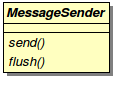
\includegraphics[scale=0.70]{images/sender.png}
            \caption{Clase \texttt{MessageSender}}
             \label{MessageSender}
        \end{figure}

        \begin{itemize}
            \item \texttt{void send(const PacketContainer\& packet\_container) = 0;}\\
                Manipula el mensaje según algún criterio para un posterior envío, o bien efectúa el envío del mensaje al
                server en el acto.
                \begin{description}
                    \item[packet\_container]: Colección de mensajes a enviar.
                \end{description}

            \item \texttt{void flush()}\\
                Fuerza el envío de mensaje en el instante que se invoca.
        \end{itemize}

    \subsubsection{\texttt{FinalSender \& ChainableSender}}

        Existen dos \textit{familias} de senders:
        \begin{itemize}
            \item \textbf{Finales:} aquellos que hacen efectivo el envío mediante una colaboración con el
                 middleware. Se implementó un sender final concreto que se llama \texttt{InmediatelySender} el
cuál envía el mensaje en el momento. Este tiene una relación con la clase \texttt{RealSender} quien se encarga
efectivamente del envío \textit{real} al servidor.
            \item \textbf{Encadenables:} no son senders finales, desconocen el middleware subyacente, por eso el
método \texttt{send} no necesariamente realiza el envío real al servidor. Estos senders pueden manipular los mensajes
con algún fin en particular antes de enviárselo al servidor.

Tienen la particularidad de que se pueden encadenar, haciendo
que cada uno luego de realizar la acción deseada le pase el mensaje al sender siguiente para que éste realice su propia
acción y así sucesivamente. Por lo tanto es decisión de cada \texttt{ChainableSender} cuando entregarle el mensaje a su
sender mas próximo. Siempre en el final de esta cadena se encontrará algun \texttt{FinalSender} concreto que hará
efectivo el envío.


     Aquí el método flush forzará pasar el mensaje al próximo sender, el cual hará lo mismo con el que sigue, llegando
en algún momento a un \texttt{FinalSender} y efectuar el envío del mensaje en el estado que se encuentre.


Un \texttt{ChainableSender} puede realizar tareas de acumulación, compresión, encriptación, etc. En el contexto de este
proyecto se realizo la implementación de un sender que acumula mensajes hasta una cantidad de $N$ bytes fijos
(\texttt{BySizeResultSender}).
                
        \end{itemize}
            \begin{figure}[!htb] \hspace{0cm}
            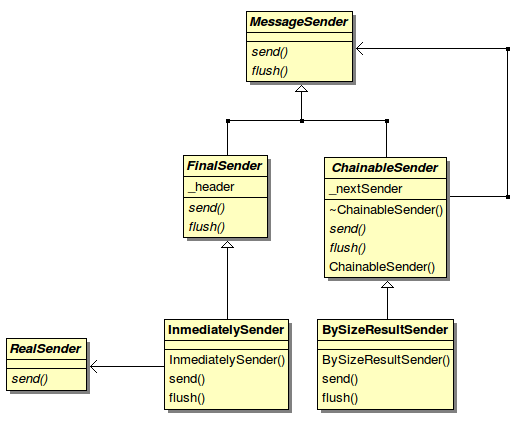
\includegraphics[scale=0.70]{images/senders.png}
            \caption{Colaboración entre los distintos \texttt{senders}}
            \label{MessageSenders}
        \end{figure}


\subsection{Asistente del cliente}

Es uno de los componentes que el usuario final podrá extender, en este caso para decirle a capa subyacente detalles de
como enviar mensajes al servidor. \rc{} al comienzo del proceso solicita al asistente del cliente el
\texttt{MessageSender} de la aplicación, por tanto se debe redefinir el método \\ \texttt{createMessageSender} con la
cadena de senders deseada o bien, dejar el asistente por defecto que encadena un sender de acumulación por bytes con
uno real.

        \begin{figure}[!htb] \hspace{2cm}
            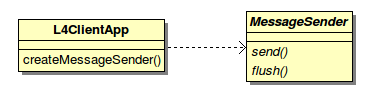
\includegraphics[scale=0.70]{images/l4_client_app.png}
            \caption{Colaboración \texttt{L4ClientApp} - \texttt{MessageSender}}
            \label{l4ca_sender}
        \end{figure}

\subsection{Política de Distribución}

Hicimos una breve introducción de este tema en \ref{distribution_policy}. Las políticas definen cuándo un cliente debe distribuir sus
unidades de trabajo pendientes o cuándo no debe y, en caso positivo, cuánto debe distribuir. El propósito de este módulo es
\textit{balancear la carga} (\textit{load balancing}, en inglés), técnica usada para compartir el trabajo a realizar entre varios recursos,
la cuál es lograda gracias a un algoritmo que divide de la manera más equitativa posible el trabajo.

% Performance
Este tipo de políticas puede influenciar mucho en la performance de una aplicación ya que el costo de comunicación en la distribución de
paquetes entre el servidor y sus clientes varía en poca o gran medida dependiendo principalmente de:
\begin{itemize}
    \item   el nivel de procesamiento que requiera la aplicación concreta en cuestión, y
    \item   de los recursos con que se cuenten (tanto en servidor como en clientes).
\end{itemize}

\subsubsection{\texttt{DistributablePolicy}}

Clase abstracta que representa cualquier política de distribución, dejando el método \texttt{how\_much\_distribute} puro virtual, el cuál
deberá ser implementado por todo usuario de la librería que desee una política ``a su gusto''.

\rc{} tiene incluido por defecto diferentes políticas de distribución, con el propósito de mostrar ``implementaciones de juguete'' y, en el
caso de la \texttt{Sigmoid}, para tener una buena política como punto de partida, la cuál fue usada en la aplicación que se dará como
ejemplo en un capítulo siguiente. En la figura \ref{distribution_policy_class} se encuentran estas políticas pre
establecidas, de las cuáles sólo
explicaremos a continuación las más relevantes.

\begin{figure}[hb]
    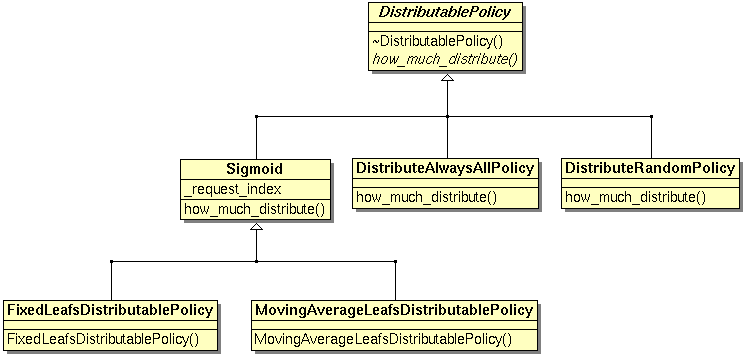
\includegraphics[scale=.6]{images/distribution_policy.png}
    \caption{Diagrama de políticas de distribución.}
    \label{distribution_policy_class}
\end{figure}

\subsubsection{\texttt{DistributeAllwaysAllPolicy}}

Está es una implementación trivial de política de distribución, y consiste en enviar siempre el máximo de unidades de trabajo que se
pueda enviar.

\subsubsection{\texttt{Sigmoid}}

Esta política describe una \textit{función sigmoidea decreciente} teniendo en cuenta el \textbf{nivel de profundidad} (en el árbol de
recursión generado por la ejecución) en el cual el functor está siendo ejecutado, ademas de las constantes: \textit{cantidad de hijos},
\textit{hojas finales} e \textit{índice de ajuste}. La fórmula que se utilizó para describir esta política es la siguiente:

\begin{center}
    \Large{$fsd(x) = \frac{children-1}{1 + e^{-(\log_{children}{leafs}) * index + x - (children-1)}} $}
\end{center}
donde:
\begin{itemize}
    \item   $children$: \textit{cantidad de hijos} que genera un functor en \textit{un} sólo paso.
    \item   $leafs$: cantidad de \textit{hojas finales} (o casos bases) que generará el cálculo completo de la aplicación corriente.
    \item   $index$: \textit{índice de ajuste}, valores altos significan más consultas al servidor sobre disponibilidad de clientes libres
            y, en contraposición, valores bajos corresponden a una mayor autosuficiencia en la ejecución de functores propios a un cliente.
\end{itemize}

El resultado de está función nos arrojará cuantos \textit{functores} podemos distribuir en relación al nivel de profundidad de manera tal
que a medida que un cliente procesa un functor con niveles cada vez más altos, el cliente distribuye menos functores y procesa más por su
cuenta. El propósito de está función es no sobrecargar al servidor de consultas sobre disponibilidad de clientes libres y la de tener un
punto (o nivel) en el cuál cada cliente sea autosuficiente en cuanto a procesamiento.

A modo de ejemplo, la figura \ref{fsi} muestra una función específica fijando la \textit{cantidad de hijos} en $8$, la cantidad de
\textit{hojas finales} en $1000$ y el \textit{índice de ajuste} en $0.5$.

\begin{figure}
    % GNUPLOT: LaTeX picture
    \setlength{\unitlength}{0.240900pt}
    \ifx\plotpoint\undefined\newsavebox{\plotpoint}\fi
    \begin{picture}(1500,900)(0,0)
    \sbox{\plotpoint}{\rule[-0.200pt]{0.400pt}{0.400pt}}%
    \put(131.0,131.0){\rule[-0.200pt]{4.818pt}{0.400pt}}
    \put(111,131){\makebox(0,0)[r]{ 0}}
    \put(1419.0,131.0){\rule[-0.200pt]{4.818pt}{0.400pt}}
    \put(131.0,228.0){\rule[-0.200pt]{4.818pt}{0.400pt}}
    \put(111,228){\makebox(0,0)[r]{ 1}}
    \put(1419.0,228.0){\rule[-0.200pt]{4.818pt}{0.400pt}}
    \put(131.0,325.0){\rule[-0.200pt]{4.818pt}{0.400pt}}
    \put(111,325){\makebox(0,0)[r]{ 2}}
    \put(1419.0,325.0){\rule[-0.200pt]{4.818pt}{0.400pt}}
    \put(131.0,422.0){\rule[-0.200pt]{4.818pt}{0.400pt}}
    \put(111,422){\makebox(0,0)[r]{ 3}}
    \put(1419.0,422.0){\rule[-0.200pt]{4.818pt}{0.400pt}}
    \put(131.0,519.0){\rule[-0.200pt]{4.818pt}{0.400pt}}
    \put(111,519){\makebox(0,0)[r]{ 4}}
    \put(1419.0,519.0){\rule[-0.200pt]{4.818pt}{0.400pt}}
    \put(131.0,616.0){\rule[-0.200pt]{4.818pt}{0.400pt}}
    \put(111,616){\makebox(0,0)[r]{ 5}}
    \put(1419.0,616.0){\rule[-0.200pt]{4.818pt}{0.400pt}}
    \put(131.0,713.0){\rule[-0.200pt]{4.818pt}{0.400pt}}
    \put(111,713){\makebox(0,0)[r]{ 6}}
    \put(1419.0,713.0){\rule[-0.200pt]{4.818pt}{0.400pt}}
    \put(131.0,810.0){\rule[-0.200pt]{4.818pt}{0.400pt}}
    \put(111,810){\makebox(0,0)[r]{ 7}}
    \put(1419.0,810.0){\rule[-0.200pt]{4.818pt}{0.400pt}}
    \put(131.0,131.0){\rule[-0.200pt]{0.400pt}{4.818pt}}
    \put(131,90){\makebox(0,0){ 0}}
    \put(131.0,839.0){\rule[-0.200pt]{0.400pt}{4.818pt}}
    \put(276.0,131.0){\rule[-0.200pt]{0.400pt}{4.818pt}}
    \put(276,90){\makebox(0,0){ 2}}
    \put(276.0,839.0){\rule[-0.200pt]{0.400pt}{4.818pt}}
    \put(422.0,131.0){\rule[-0.200pt]{0.400pt}{4.818pt}}
    \put(422,90){\makebox(0,0){ 4}}
    \put(422.0,839.0){\rule[-0.200pt]{0.400pt}{4.818pt}}
    \put(567.0,131.0){\rule[-0.200pt]{0.400pt}{4.818pt}}
    \put(567,90){\makebox(0,0){ 6}}
    \put(567.0,839.0){\rule[-0.200pt]{0.400pt}{4.818pt}}
    \put(712.0,131.0){\rule[-0.200pt]{0.400pt}{4.818pt}}
    \put(712,90){\makebox(0,0){ 8}}
    \put(712.0,839.0){\rule[-0.200pt]{0.400pt}{4.818pt}}
    \put(858.0,131.0){\rule[-0.200pt]{0.400pt}{4.818pt}}
    \put(858,90){\makebox(0,0){ 10}}
    \put(858.0,839.0){\rule[-0.200pt]{0.400pt}{4.818pt}}
    \put(1003.0,131.0){\rule[-0.200pt]{0.400pt}{4.818pt}}
    \put(1003,90){\makebox(0,0){ 12}}
    \put(1003.0,839.0){\rule[-0.200pt]{0.400pt}{4.818pt}}
    \put(1148.0,131.0){\rule[-0.200pt]{0.400pt}{4.818pt}}
    \put(1148,90){\makebox(0,0){ 14}}
    \put(1148.0,839.0){\rule[-0.200pt]{0.400pt}{4.818pt}}
    \put(1294.0,131.0){\rule[-0.200pt]{0.400pt}{4.818pt}}
    \put(1294,90){\makebox(0,0){ 16}}
    \put(1294.0,839.0){\rule[-0.200pt]{0.400pt}{4.818pt}}
    \put(1439.0,131.0){\rule[-0.200pt]{0.400pt}{4.818pt}}
    \put(1439,90){\makebox(0,0){ 18}}
    \put(1439.0,839.0){\rule[-0.200pt]{0.400pt}{4.818pt}}
    \put(131.0,131.0){\rule[-0.200pt]{0.400pt}{175.375pt}}
    \put(131.0,131.0){\rule[-0.200pt]{315.097pt}{0.400pt}}
    \put(1439.0,131.0){\rule[-0.200pt]{0.400pt}{175.375pt}}
    \put(131.0,859.0){\rule[-0.200pt]{315.097pt}{0.400pt}}
    \put(30,495){\makebox(0,0){f(x)}}
    \put(785,29){\makebox(0,0){x}}
    % \put(1279,819){\makebox(0,0)[r]{7 / (1 + exp(-((log(1000)/log(8)) * 0.5)+x-7))}}
    % \put(1299.0,819.0){\rule[-0.200pt]{24.090pt}{0.400pt}}
    \put(131,810){\usebox{\plotpoint}}
    \put(276,808.67){\rule{3.373pt}{0.400pt}}
    \multiput(276.00,809.17)(7.000,-1.000){2}{\rule{1.686pt}{0.400pt}}
    \put(131.0,810.0){\rule[-0.200pt]{34.930pt}{0.400pt}}
    \put(329,807.67){\rule{3.132pt}{0.400pt}}
    \multiput(329.00,808.17)(6.500,-1.000){2}{\rule{1.566pt}{0.400pt}}
    \put(290.0,809.0){\rule[-0.200pt]{9.395pt}{0.400pt}}
    \put(356,806.67){\rule{3.132pt}{0.400pt}}
    \multiput(356.00,807.17)(6.500,-1.000){2}{\rule{1.566pt}{0.400pt}}
    \put(342.0,808.0){\rule[-0.200pt]{3.373pt}{0.400pt}}
    \put(382,805.67){\rule{3.132pt}{0.400pt}}
    \multiput(382.00,806.17)(6.500,-1.000){2}{\rule{1.566pt}{0.400pt}}
    \put(395,804.67){\rule{3.132pt}{0.400pt}}
    \multiput(395.00,805.17)(6.500,-1.000){2}{\rule{1.566pt}{0.400pt}}
    \put(408,803.67){\rule{3.373pt}{0.400pt}}
    \multiput(408.00,804.17)(7.000,-1.000){2}{\rule{1.686pt}{0.400pt}}
    \put(422,802.67){\rule{3.132pt}{0.400pt}}
    \multiput(422.00,803.17)(6.500,-1.000){2}{\rule{1.566pt}{0.400pt}}
    \put(435,801.17){\rule{2.700pt}{0.400pt}}
    \multiput(435.00,802.17)(7.396,-2.000){2}{\rule{1.350pt}{0.400pt}}
    \put(448,799.67){\rule{3.132pt}{0.400pt}}
    \multiput(448.00,800.17)(6.500,-1.000){2}{\rule{1.566pt}{0.400pt}}
    \multiput(461.00,798.95)(2.918,-0.447){3}{\rule{1.967pt}{0.108pt}}
    \multiput(461.00,799.17)(9.918,-3.000){2}{\rule{0.983pt}{0.400pt}}
    \put(475,795.17){\rule{2.700pt}{0.400pt}}
    \multiput(475.00,796.17)(7.396,-2.000){2}{\rule{1.350pt}{0.400pt}}
    \multiput(488.00,793.95)(2.695,-0.447){3}{\rule{1.833pt}{0.108pt}}
    \multiput(488.00,794.17)(9.195,-3.000){2}{\rule{0.917pt}{0.400pt}}
    \multiput(501.00,790.94)(1.797,-0.468){5}{\rule{1.400pt}{0.113pt}}
    \multiput(501.00,791.17)(10.094,-4.000){2}{\rule{0.700pt}{0.400pt}}
    \multiput(514.00,786.94)(1.797,-0.468){5}{\rule{1.400pt}{0.113pt}}
    \multiput(514.00,787.17)(10.094,-4.000){2}{\rule{0.700pt}{0.400pt}}
    \multiput(527.00,782.93)(1.489,-0.477){7}{\rule{1.220pt}{0.115pt}}
    \multiput(527.00,783.17)(11.468,-5.000){2}{\rule{0.610pt}{0.400pt}}
    \multiput(541.00,777.93)(1.123,-0.482){9}{\rule{0.967pt}{0.116pt}}
    \multiput(541.00,778.17)(10.994,-6.000){2}{\rule{0.483pt}{0.400pt}}
    \multiput(554.00,771.93)(0.950,-0.485){11}{\rule{0.843pt}{0.117pt}}
    \multiput(554.00,772.17)(11.251,-7.000){2}{\rule{0.421pt}{0.400pt}}
    \multiput(567.00,764.93)(0.824,-0.488){13}{\rule{0.750pt}{0.117pt}}
    \multiput(567.00,765.17)(11.443,-8.000){2}{\rule{0.375pt}{0.400pt}}
    \multiput(580.00,756.92)(0.652,-0.491){17}{\rule{0.620pt}{0.118pt}}
    \multiput(580.00,757.17)(11.713,-10.000){2}{\rule{0.310pt}{0.400pt}}
    \multiput(593.00,746.92)(0.637,-0.492){19}{\rule{0.609pt}{0.118pt}}
    \multiput(593.00,747.17)(12.736,-11.000){2}{\rule{0.305pt}{0.400pt}}
    \multiput(607.00,735.92)(0.539,-0.492){21}{\rule{0.533pt}{0.119pt}}
    \multiput(607.00,736.17)(11.893,-12.000){2}{\rule{0.267pt}{0.400pt}}
    \multiput(620.58,722.67)(0.493,-0.576){23}{\rule{0.119pt}{0.562pt}}
    \multiput(619.17,723.83)(13.000,-13.834){2}{\rule{0.400pt}{0.281pt}}
    \multiput(633.58,707.41)(0.493,-0.655){23}{\rule{0.119pt}{0.623pt}}
    \multiput(632.17,708.71)(13.000,-15.707){2}{\rule{0.400pt}{0.312pt}}
    \multiput(646.58,690.29)(0.493,-0.695){23}{\rule{0.119pt}{0.654pt}}
    \multiput(645.17,691.64)(13.000,-16.643){2}{\rule{0.400pt}{0.327pt}}
    \multiput(659.58,672.09)(0.494,-0.754){25}{\rule{0.119pt}{0.700pt}}
    \multiput(658.17,673.55)(14.000,-19.547){2}{\rule{0.400pt}{0.350pt}}
    \multiput(673.58,650.65)(0.493,-0.893){23}{\rule{0.119pt}{0.808pt}}
    \multiput(672.17,652.32)(13.000,-21.324){2}{\rule{0.400pt}{0.404pt}}
    \multiput(686.58,627.39)(0.493,-0.972){23}{\rule{0.119pt}{0.869pt}}
    \multiput(685.17,629.20)(13.000,-23.196){2}{\rule{0.400pt}{0.435pt}}
    \multiput(699.58,602.14)(0.493,-1.052){23}{\rule{0.119pt}{0.931pt}}
    \multiput(698.17,604.07)(13.000,-25.068){2}{\rule{0.400pt}{0.465pt}}
    \multiput(712.58,575.26)(0.494,-1.011){25}{\rule{0.119pt}{0.900pt}}
    \multiput(711.17,577.13)(14.000,-26.132){2}{\rule{0.400pt}{0.450pt}}
    \multiput(726.58,546.75)(0.493,-1.171){23}{\rule{0.119pt}{1.023pt}}
    \multiput(725.17,548.88)(13.000,-27.877){2}{\rule{0.400pt}{0.512pt}}
    \multiput(739.58,516.63)(0.493,-1.210){23}{\rule{0.119pt}{1.054pt}}
    \multiput(738.17,518.81)(13.000,-28.813){2}{\rule{0.400pt}{0.527pt}}
    \multiput(752.58,485.63)(0.493,-1.210){23}{\rule{0.119pt}{1.054pt}}
    \multiput(751.17,487.81)(13.000,-28.813){2}{\rule{0.400pt}{0.527pt}}
    \multiput(765.58,454.75)(0.493,-1.171){23}{\rule{0.119pt}{1.023pt}}
    \multiput(764.17,456.88)(13.000,-27.877){2}{\rule{0.400pt}{0.512pt}}
    \multiput(778.58,425.03)(0.494,-1.084){25}{\rule{0.119pt}{0.957pt}}
    \multiput(777.17,427.01)(14.000,-28.013){2}{\rule{0.400pt}{0.479pt}}
    \multiput(792.58,394.88)(0.493,-1.131){23}{\rule{0.119pt}{0.992pt}}
    \multiput(791.17,396.94)(13.000,-26.940){2}{\rule{0.400pt}{0.496pt}}
    \multiput(805.58,366.14)(0.493,-1.052){23}{\rule{0.119pt}{0.931pt}}
    \multiput(804.17,368.07)(13.000,-25.068){2}{\rule{0.400pt}{0.465pt}}
    \multiput(818.58,339.26)(0.493,-1.012){23}{\rule{0.119pt}{0.900pt}}
    \multiput(817.17,341.13)(13.000,-24.132){2}{\rule{0.400pt}{0.450pt}}
    \multiput(831.58,313.65)(0.493,-0.893){23}{\rule{0.119pt}{0.808pt}}
    \multiput(830.17,315.32)(13.000,-21.324){2}{\rule{0.400pt}{0.404pt}}
    \multiput(844.58,290.98)(0.494,-0.791){25}{\rule{0.119pt}{0.729pt}}
    \multiput(843.17,292.49)(14.000,-20.488){2}{\rule{0.400pt}{0.364pt}}
    \multiput(858.58,269.16)(0.493,-0.734){23}{\rule{0.119pt}{0.685pt}}
    \multiput(857.17,270.58)(13.000,-17.579){2}{\rule{0.400pt}{0.342pt}}
    \multiput(871.58,250.41)(0.493,-0.655){23}{\rule{0.119pt}{0.623pt}}
    \multiput(870.17,251.71)(13.000,-15.707){2}{\rule{0.400pt}{0.312pt}}
    \multiput(884.58,233.67)(0.493,-0.576){23}{\rule{0.119pt}{0.562pt}}
    \multiput(883.17,234.83)(13.000,-13.834){2}{\rule{0.400pt}{0.281pt}}
    \multiput(897.00,219.92)(0.497,-0.494){25}{\rule{0.500pt}{0.119pt}}
    \multiput(897.00,220.17)(12.962,-14.000){2}{\rule{0.250pt}{0.400pt}}
    \multiput(911.00,205.92)(0.590,-0.492){19}{\rule{0.573pt}{0.118pt}}
    \multiput(911.00,206.17)(11.811,-11.000){2}{\rule{0.286pt}{0.400pt}}
    \multiput(924.00,194.92)(0.652,-0.491){17}{\rule{0.620pt}{0.118pt}}
    \multiput(924.00,195.17)(11.713,-10.000){2}{\rule{0.310pt}{0.400pt}}
    \multiput(937.00,184.93)(0.728,-0.489){15}{\rule{0.678pt}{0.118pt}}
    \multiput(937.00,185.17)(11.593,-9.000){2}{\rule{0.339pt}{0.400pt}}
    \multiput(950.00,175.93)(0.950,-0.485){11}{\rule{0.843pt}{0.117pt}}
    \multiput(950.00,176.17)(11.251,-7.000){2}{\rule{0.421pt}{0.400pt}}
    \multiput(963.00,168.93)(1.214,-0.482){9}{\rule{1.033pt}{0.116pt}}
    \multiput(963.00,169.17)(11.855,-6.000){2}{\rule{0.517pt}{0.400pt}}
    \multiput(977.00,162.93)(1.378,-0.477){7}{\rule{1.140pt}{0.115pt}}
    \multiput(977.00,163.17)(10.634,-5.000){2}{\rule{0.570pt}{0.400pt}}
    \multiput(990.00,157.93)(1.378,-0.477){7}{\rule{1.140pt}{0.115pt}}
    \multiput(990.00,158.17)(10.634,-5.000){2}{\rule{0.570pt}{0.400pt}}
    \multiput(1003.00,152.95)(2.695,-0.447){3}{\rule{1.833pt}{0.108pt}}
    \multiput(1003.00,153.17)(9.195,-3.000){2}{\rule{0.917pt}{0.400pt}}
    \multiput(1016.00,149.94)(1.797,-0.468){5}{\rule{1.400pt}{0.113pt}}
    \multiput(1016.00,150.17)(10.094,-4.000){2}{\rule{0.700pt}{0.400pt}}
    \put(1029,145.17){\rule{2.900pt}{0.400pt}}
    \multiput(1029.00,146.17)(7.981,-2.000){2}{\rule{1.450pt}{0.400pt}}
    \multiput(1043.00,143.95)(2.695,-0.447){3}{\rule{1.833pt}{0.108pt}}
    \multiput(1043.00,144.17)(9.195,-3.000){2}{\rule{0.917pt}{0.400pt}}
    \put(1056,140.67){\rule{3.132pt}{0.400pt}}
    \multiput(1056.00,141.17)(6.500,-1.000){2}{\rule{1.566pt}{0.400pt}}
    \put(1069,139.17){\rule{2.700pt}{0.400pt}}
    \multiput(1069.00,140.17)(7.396,-2.000){2}{\rule{1.350pt}{0.400pt}}
    \put(1082,137.67){\rule{3.132pt}{0.400pt}}
    \multiput(1082.00,138.17)(6.500,-1.000){2}{\rule{1.566pt}{0.400pt}}
    \put(1095,136.67){\rule{3.373pt}{0.400pt}}
    \multiput(1095.00,137.17)(7.000,-1.000){2}{\rule{1.686pt}{0.400pt}}
    \put(1109,135.67){\rule{3.132pt}{0.400pt}}
    \multiput(1109.00,136.17)(6.500,-1.000){2}{\rule{1.566pt}{0.400pt}}
    \put(1122,134.67){\rule{3.132pt}{0.400pt}}
    \multiput(1122.00,135.17)(6.500,-1.000){2}{\rule{1.566pt}{0.400pt}}
    \put(1135,133.67){\rule{3.132pt}{0.400pt}}
    \multiput(1135.00,134.17)(6.500,-1.000){2}{\rule{1.566pt}{0.400pt}}
    \put(369.0,807.0){\rule[-0.200pt]{3.132pt}{0.400pt}}
    \put(1162,132.67){\rule{3.132pt}{0.400pt}}
    \multiput(1162.00,133.17)(6.500,-1.000){2}{\rule{1.566pt}{0.400pt}}
    \put(1148.0,134.0){\rule[-0.200pt]{3.373pt}{0.400pt}}
    \put(1201,131.67){\rule{3.132pt}{0.400pt}}
    \multiput(1201.00,132.17)(6.500,-1.000){2}{\rule{1.566pt}{0.400pt}}
    \put(1175.0,133.0){\rule[-0.200pt]{6.263pt}{0.400pt}}
    \put(1280,130.67){\rule{3.373pt}{0.400pt}}
    \multiput(1280.00,131.17)(7.000,-1.000){2}{\rule{1.686pt}{0.400pt}}
    \put(1214.0,132.0){\rule[-0.200pt]{15.899pt}{0.400pt}}
    \put(1294.0,131.0){\rule[-0.200pt]{34.930pt}{0.400pt}}
    \put(131.0,131.0){\rule[-0.200pt]{0.400pt}{175.375pt}}
    \put(131.0,131.0){\rule[-0.200pt]{315.097pt}{0.400pt}}
    \put(1439.0,131.0){\rule[-0.200pt]{0.400pt}{175.375pt}}
    \put(131.0,859.0){\rule[-0.200pt]{315.097pt}{0.400pt}}
    \end{picture}
    \caption{Función sigmoidea decreciente con $children=8$, $leafs=1000$ e $index=0.5$.}
    \label{fsi}
\end{figure}
